\documentclass[letterpaper]{article}
\PassOptionsToPackage{table}{xcolor}
\usepackage[submission]{aaai2027}
\nocopyright
\usepackage[hyphens]{url}
\usepackage{graphicx}
\urlstyle{rm}
\def\UrlFont{\rm}
\usepackage{natbib}
\usepackage{caption}
\frenchspacing

\usepackage{amsmath,amssymb}
\usepackage{booktabs}
\usepackage{array}
\usepackage{tabularx}
\usepackage{makecell}
\usepackage{multirow}

\pdfinfo{
/TemplateVersion (2027.1)
}

\setcounter{secnumdepth}{1}
\newcolumntype{Y}{>{\centering\arraybackslash}X}

\title{One Ocean, Many Tasks: Supplementary Appendix}
\author{Anonymous Submission}
\affiliations{}

\begin{document}
\maketitle

\noindent\textbf{Paper ID:} 6895\par
\noindent This appendix details the environment representation, task objectives, motion and pollution models, and evaluation protocol. It also reports complementary studies of dynamics, disturbance strength, planner decisions, and scene-backed multi-agent behavior.

\appendix
\renewcommand{\thefigure}{A\arabic{figure}}
\renewcommand{\thetable}{A\arabic{table}}
\renewcommand{\theequation}{A\arabic{equation}}
\section{Ocean Dataset and Validation}
\label{app:data}

\subsection{Sources, harmonization, and schema}

OneOcean combines bathymetry from the General Bathymetric Chart of the Oceans (GEBCO) \cite{GEBCO2025} with horizontal currents from the Copernicus Marine Service Global Ocean Physics Analysis and Forecast (GOPAF) product \cite{copernicus,CopernicusGOPAF2025}. The resulting Network Common Data Form (NetCDF) product is harmonized by cropping the requested region, retaining returned time and depth coordinates, normalizing coordinate names and units, interpolating variables onto one latitude--longitude grid, preserving invalid terrain and NoData cells, and recording the transformations.

\begin{figure*}[t]
\centering
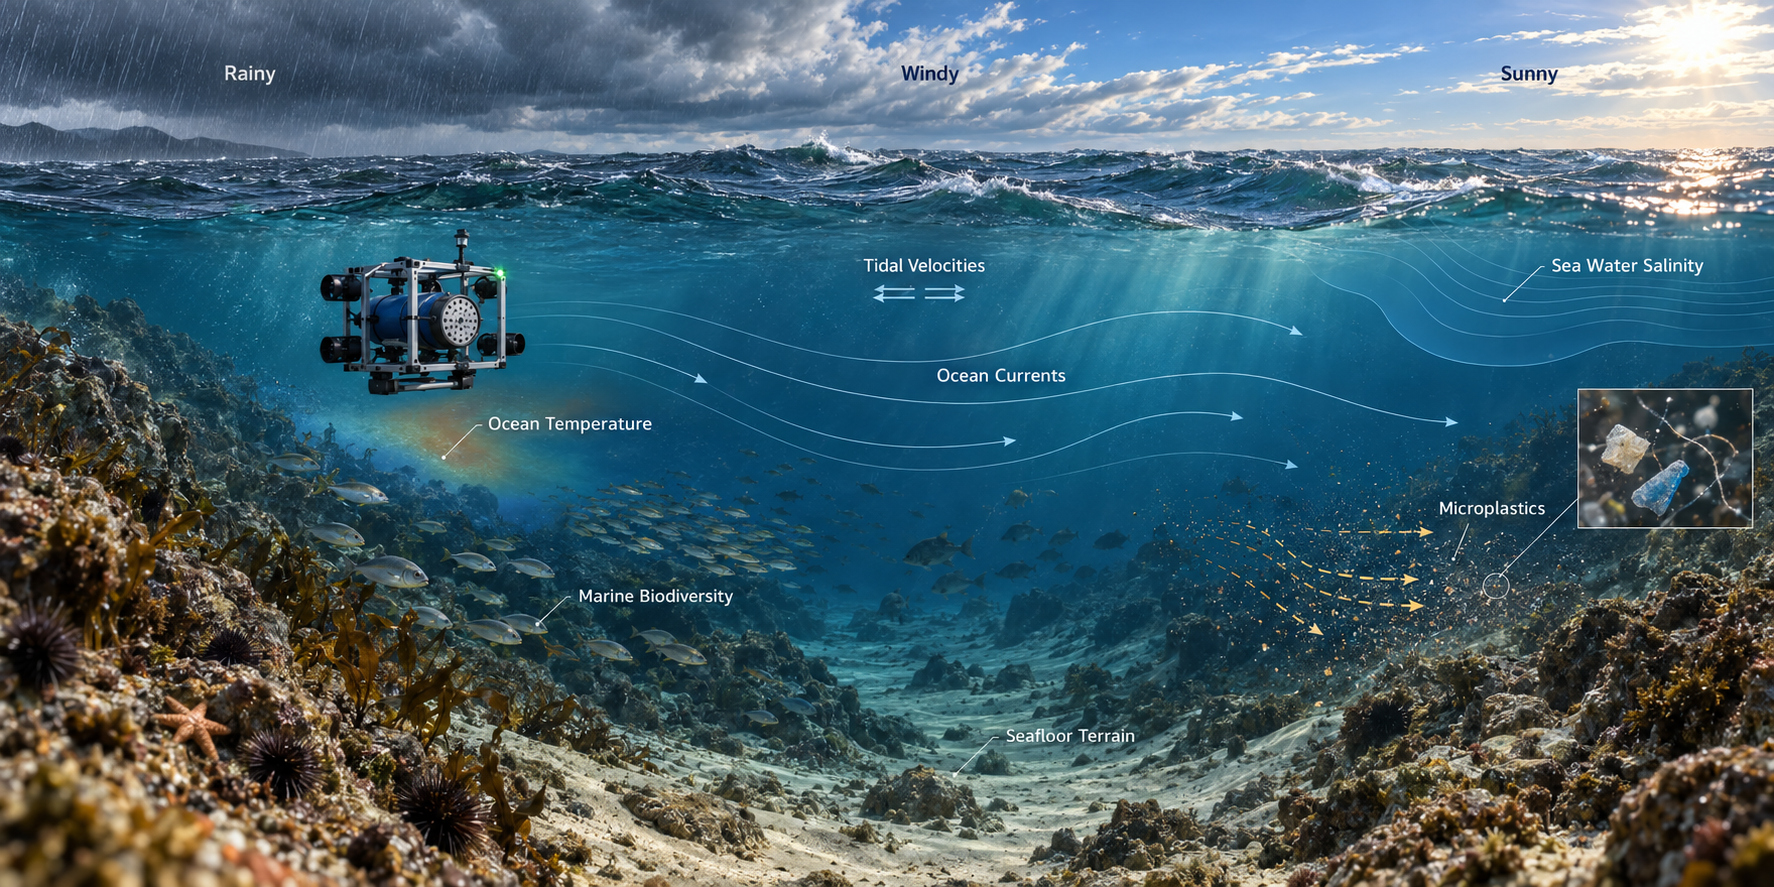
\includegraphics[width=0.98\textwidth]{figures/overview2.jpg}
\caption{Conceptual overview of ocean conditions and ecological signals relevant to OneOcean, including terrain, currents, tides, temperature, salinity, weather, biodiversity, and microplastics.}
\label{fig:app_environment_overview}
\end{figure*}

\begin{table*}[t]
\centering
\scriptsize
\setlength{\tabcolsep}{4pt}
\renewcommand{\arraystretch}{1.10}
\begin{tabularx}{\textwidth}{l l l X}
\toprule
\textbf{Canonical field} & \textbf{Dimensions} & \textbf{Unit or Encoding} & \textbf{Contract} \\
\midrule
Latitude & $H$ & degrees north & Strictly monotonic geographic coordinate. \\
Longitude & $W$ & degrees east & Strictly monotonic geographic coordinate. \\
Time & $T$ & Climate and Forecast time unit & Monotonic timestamps retained from the source product. \\
Depth & $D$ & m, positive down & Actual depth coordinates returned by the source. \\
Eastward and northward current & $T\!\times\!D\!\times\!H\!\times\!W$ & m\,s$^{-1}$ & Base pair $(u,v)$ or tide-combined pair $(u_{\mathrm{total}},v_{\mathrm{total}})$. \\
Elevation & $H\!\times\!W$ & m relative to sea surface & Bathymetric elevation aligned to the current grid. \\
Validity mask & $H\!\times\!W$ & binary & Invalid terrain, crop-exterior, or NoData cells. \\
\bottomrule
\end{tabularx}
\caption{Canonical environment-product schema. The validator accepts documented aliases but maps every accepted product to these semantics.}
\label{tab:app_data_contract}
\end{table*}

Masked elevation cells use zero as a storage fill value; elevation is interpreted together with the validity mask. In the core simulation frame, $(x,y,z)=$(east, depth-down, north), and the dataset vector $(u,v)$ maps to $(u,0,v)$. Longitude and latitude are converted to local metric $x$ and $z$ about the recorded lower-left geographic origin.

\subsection{Depth and tide treatment}

The realized \texttt{tiny} request contains one level at 0.494\,m. The \texttt{scene} and \texttt{public} requests cover 0--200\,m and retain 26 source levels from 0.494 to 186.126\,m. The pipeline retains the returned depth coordinates. Consequently, \texttt{tiny} is a time-varying 2D or 2.5D current product, whereas the other two products provide source-derived horizontal current at multiple discrete depths.

Only the current \texttt{scene} release includes tide components. Hourly tide samples are aligned to the base product with nearest-time selection and attenuated as $\exp(-d/z_0)$ with $z_0=50$\,m before forming the total current pair. The exported temporal resolution follows the base-product clock; coarse time sampling removes higher-frequency variation.

\subsection{Dataset validation}

The release validator checks required fields, aliases, dimensions, monotonic coordinates, units, finite sampled values, mask semantics, provenance, and optional round-trip fidelity between NetCDF and a NumPy Archive (NPZ). Table~\ref{tab:app_validator} summarizes the July 21, 2026 validation of the released products.

\begin{table}[t]
\centering
\scriptsize
\setlength{\tabcolsep}{3pt}
\renewcommand{\arraystretch}{1.10}
\begin{tabularx}{\columnwidth}{l X c c l}
\toprule
\textbf{Variant} & \textbf{Current pair} & \textbf{Errors} & \textbf{Warn.} & \textbf{Round-trip} \\
\midrule
\texttt{tiny} & \texttt{uo}, \texttt{vo} & 0 & 3 & Exact \\
\texttt{scene} & \texttt{utotal}, \texttt{vtotal} & 0 & 4 & Not run \\
\texttt{public} & \texttt{uo}, \texttt{vo} & 0 & 2 & Not run \\
\bottomrule
\end{tabularx}
\caption{Environment-product validation. All variants are \texttt{PASS\_WITH\_WARNINGS}; the metadata warnings are listed below. Round-trip denotes the fixed \texttt{tiny} $(t=0,d=0)$ NetCDF-to-NPZ check.}
\label{tab:app_validator}
\end{table}

The warnings identify missing depth or elevation units, total-current units, or mask flag meanings depending on the variant. Regeneration with the updated pipeline writes these attributes. The tested \texttt{tiny} slice preserved coordinates and currents at absolute tolerance $10^{-6}$.

\subsection{Portable provenance}

Every regenerated NetCDF records source product identifiers, requested and actual region, time, and depth, tide inclusion and depth profile, interpolation and missing-value handling, and generation software. Companion variant manifests use paths relative to the variant directory. Each run records the selected time and depth indices.

\subsection{Geographic sampling within an episode}

Let $(\phi_0,\lambda_0)$ be an episode's geographic origin and $p=(x,y,z)$ its local position in meters. The core sampler uses
\begin{align}
\phi(p)&=\phi_0+z/L,\\
\lambda(p)&=\lambda_0+x/[L\max(0.1,\cos\phi_0)],
\end{align}
where $L=111132$\,m per degree and the cosine evaluates latitude in radians. At reset, the origin is sampled within the available geographic extent to place the simulation tile on the environmental grid. The default tile spans $600\times600$\,m horizontally, with vehicle depth bounded between 2 and 18\,m. Environmental coordinates retain the source grid spacing.

For grid coordinates $\{\phi_j\}$ and $\{\lambda_k\}$, the sampled indices are
\begin{equation}
j^*=\arg\min_j|\phi_j-\phi(p)|,\qquad
k^*=\arg\min_k|\lambda_k-\lambda(p)|.
\end{equation}
The current at $p$ is $g(u_{j^*k^*},0,v_{j^*k^*})$, where $g$ is the current gain. Bathymetry and validity use the same indices. Missing current samples are set to zero, while terrain feasibility is determined separately by the validity mask and seabed clearance. Core episodes query a fixed time and depth slice.

\subsection{Temporal forcing in the scene backend}

The scene backend uses an exported current sequence at a selected geographic location and the nearest available source depth. Let $T_c$ be its number of temporal samples, $s$ the episode seed, and $\alpha$ the configured sequence-advance rate. At simulation time $t$, the sampled index is
\begin{equation}
i(t)=\big[(s\bmod T_c)+\lfloor\alpha t\rfloor\big]\bmod T_c.
\end{equation}
Setting $\alpha=0$ holds the initial sample; a positive value advances the sequence and wraps at its end. For a daily export, $\alpha$ gives source days per simulated second. The sampled vector, multiplied by the current gain, drives the scene disturbance. Spatial slices and temporal sequences provide complementary conditions for evaluating disturbance rejection.

\section{Task Definitions}
\label{app:tasks}

Every task declares its objective, observations, feasibility constraints, success condition, and primary metric. Shared observations include pose and relative target cues, local current, and task-specific probes; shared feasibility checks include domain bounds, terrain validity, seafloor clearance, and configured team size.

\begin{description}
\item[Go-to-Goal Under Currents (G2G).] Reach a goal while rejecting data-grounded drift; success requires entering the goal tolerance, and final goal error is primary.
\item[Station Keeping (SK).] Hold position under disturbance; station RMS error measures sustained deviation.
\item[Route Following (RF).] Visit an ordered waypoint route; cross-track error and reached waypoints expose partial progress.
\item[Depth-Profile Tracking (DPT).] Follow a target depth profile during motion; depth-tracking error is primary.
\item[Area Scan (AS).] Cover a bounded region over 3D terrain; grid coverage fraction measures progress.
\item[Pipeline Inspection (PI).] Follow a pipeline corridor and encounter leak cues; the inspection score is the detected-leak fraction, with route progress recorded separately.
\item[Formation Transit (FT).] Move a team of 2--10 vehicles while maintaining relative geometry; formation error and collision ratio capture coordination quality.
\item[Surface Pollution Cleanup (SPC).] Assign 2--10 vehicles to discrete surface sources and satisfy per-source dwell requirements; cleanup rate is completed-source fraction.
\item[Underwater Pollution Lift (UPL).] Coordinate five vehicles around a payload and lift it to the surface; lift completion defines success.
\item[Fish Protection / Herding (FH).] Use eight vehicles to contain and escort a fish school under currents; centroid progress toward the escort goal defines success.
\end{description}

\subsection{Exact progress metrics}

Several task metrics are normalized ratios with distinct denominators. Let $\mathcal V$ be the visited scan cells in an $H\times W$ grid, $N_{\mathrm{det}}$ the detected leaks among $N_{\mathrm{leak}}$ placed leaks, and $N_{\mathrm{done}}$ the sources whose dwell requirement is complete among $N_{\mathrm{src}}$ sources. The released evaluator computes
\begin{align}
\mathrm{Cov}_{\mathrm{AS}}
  &= \frac{|\mathcal V|}{HW}, \label{eq:as_progress}\\
\mathrm{Score}_{\mathrm{PI}}
  &= \frac{N_{\mathrm{det}}}{N_{\mathrm{leak}}}, \label{eq:pi_progress}\\
\mathrm{Rate}_{\mathrm{SPC}}
  &= \frac{N_{\mathrm{done}}}{N_{\mathrm{src}}}, \label{eq:spc_progress}\\
e_{\mathrm{FT}}
  &= \frac{1}{N}\sum_{i=1}^{N}
     \left\|p_i-(p_g+r_i)\right\|_2, \label{eq:ft_error}\\
\mathrm{Prog}_{\mathrm{FH}}(t)
  &= \operatorname{clip}\!\left(1-\frac{d_t}{d_0},0,1\right). \label{eq:fh_progress}
\end{align}
Here $p_g+r_i$ is agent $i$'s assigned formation goal, while $d_t$ and $d_0$ are the current and initial fish-centroid distances to the escort goal. Each task reports its own progress metric.

Tiers 1, 2, and 3 preserve the task definitions. Each tier specifies a joint setting of current gain, tolerances, route or coverage extent, sensing difficulty, and coordination requirements. Navigation and tracking tasks primarily stress disturbance rejection, sensing and inspection tasks stress spatial coverage and event encounters, and coordination and pollution tasks add team geometry, assignment, or dwell-time coupling.

\subsection{State-dependent completion}

\paragraph{Navigation and station keeping.}
Let $d_n=\min_i\|p_i^n-p_g\|_2$. G2G completes when $d_n$ enters the goal radius. SK requires consecutive qualifying steps: its hold counter follows
\begin{equation}
h_{n+1}=\begin{cases}h_n+1,&d_n\leq r,\\0,&d_n>r.\end{cases}
\end{equation}
Success occurs when $h_{n+1}$ reaches the prescribed hold length. Consequently, an excursion outside the station radius restarts the hold interval. RF and DPT maintain an ordered waypoint index, advance it when a vehicle enters the active waypoint radius, and evaluate completion from the updated index and that step's waypoint distance. DPT additionally requires the team-mean absolute depth error relative to the evaluated waypoint to satisfy its depth tolerance. FT applies its tolerance to every assigned formation goal: $\max_i\|p_i-(p_g+r_i)\|_2\leq r$.

\paragraph{Area coverage and inspection.}
AS stores a persistent binary grid of visited cells. With sensor radius $r_s$ and cell width $\ell$, a vehicle marks a square neighborhood extending $\lfloor r_s/\ell\rfloor$ cells in each horizontal direction, clipped at the grid boundary. Cells are counted once. A lawnmower route supplies intermediate goals, while completion depends on the coverage fraction in Equation~\ref{eq:as_progress}. PI maintains a separate detection flag for each leak. A flag becomes permanent when any vehicle enters the leak's detection radius; the first encounter time is recorded. Detection of all leaks completes the task, and the waypoint index records traversal progress separately.

\paragraph{Accumulated service in surface cleanup.}
For source $j$, let $a_i^n$ denote agent $i$'s assigned source and $q$ the required number of agents. Its accumulated service time is
\begin{align}
b_j^n&=\sum_i\mathbf 1[a_i^n=j]\,
                 \mathbf 1[\|p_i^n-s_j\|_2\leq r],\\
\tau_j^{n+1}&=\tau_j^n+\Delta t\,\mathbf 1[b_j^n\geq q].
\end{align}
A source completes when $\tau_j$ reaches its dwell threshold. Service already accumulated is retained when vehicles leave; this differs from the consecutive hold in SK. Only vehicles assigned to that source contribute to its service count. The task completes once every source is finished. The hard preset couples assignment with rendezvous by requiring two agents to service a source simultaneously.

\paragraph{Attachment and collective lifting.}
UPL has four phases: approach, lift-off, fifth-agent joining, and ascent. Each of the five agents acquires a persistent attachment flag upon entering the payload attachment radius. Attachment of the first four agents starts the lift-off hold; completing that hold enables joining, and attachment of the fifth agent enables ascent. During the lifting phases the payload follows the attached team's mean position with a phase-dependent depth update. Completion requires the ascent phase, all five attachments, and payload depth at or above the designated surface threshold.

\paragraph{Fish-school escort.}
FH evolves a school under current drift and a herding response to nearby vehicles. Its progress uses the horizontal distance between the school centroid and escort goal. The eight-vehicle team succeeds when either the normalized progress in Equation~\ref{eq:fh_progress} reaches its target or the centroid enters the goal radius.

\begin{table*}[t]
\centering\scriptsize
\setlength{\tabcolsep}{4pt}
\renewcommand{\arraystretch}{1.13}
\begin{tabularx}{\textwidth}{l X X r r}
\toprule
\textbf{Task} & \textbf{Tier 2 parameters} & \textbf{Tier 3 parameters} & \multicolumn{2}{c}{\textbf{Step budget}}\\
 & & & \textbf{Tier 2} & \textbf{Tier 3}\\
\midrule
G2G & Goal radius 4\,m & Goal radius 1.3\,m & 280 & 300\\
SK & Radius 2.6\,m; hold 110 steps & Radius 1.3\,m; hold 240 steps & 360 & 560\\
RF & 12 waypoints; radius 3.2\,m & 20 waypoints; radius 1.6\,m & 460 & 560\\
DPT & 12 waypoints; radius 3.6\,m; depth tolerance 1.2\,m & 18 waypoints; radius 1.8\,m; depth tolerance 0.7\,m & 560 & 720\\
FT & Formation radius 36\,m; goal tolerance 4\,m & Formation radius 70\,m; goal tolerance 1\,m & 600 & 550\\
SPC & 12 sources; radius 3.8\,m; dwell 8\,s; one agent & 6 sources; radius 2.6\,m; dwell 6\,s; two agents & 720 & 900\\
UPL & Attach radius 4\,m; hold 3.5\,s; surface depth 2.5\,m & Attach radius 3\,m; hold 4\,s; surface depth 2.5\,m & 720 & 880\\
FH & 220 fish; progress 0.995 or goal radius 12\,m & 160 fish; progress 0.99 or goal radius 7\,m & 650 & 900\\
AS & Cell 75\,m; sensor radius 35\,m; coverage 0.82 & Cell 60\,m; sensor radius 70\,m; coverage 0.95 & 2000 & 1700\\
PI & 14 waypoints; 6 leaks; detection radius 5\,m & 20 waypoints; 8 leaks; detection radius 3.6\,m & 1500 & 1500\\
\bottomrule
\end{tabularx}
\caption{Task-specific parameters for the two principal evaluation tiers. Durations follow from the step budget and simulation timestep; the default $\Delta t$ is 1\,s. UPL uses five vehicles and FH uses eight.}
\label{tab:app_task_thresholds}
\end{table*}

\section{Implementation Defaults, Pollution, and ROS 2}
\label{app:models_ros}

\subsection{Dynamics parameters}

The main paper defines current coupling, action clipping, diagonal vehicle dynamics, and terrain feasibility. Table~\ref{tab:app_dynamics_defaults} lists the Six-Degree-of-Freedom (6DoF) parameters recorded in each run specification.

\begin{table*}[t]
\centering
\scriptsize
\setlength{\tabcolsep}{4pt}
\renewcommand{\arraystretch}{1.08}
\begin{tabularx}{\textwidth}{l r X l r X}
\toprule
\textbf{Field} & \textbf{Default} & \textbf{Meaning} & \textbf{Field} & \textbf{Default} & \textbf{Meaning} \\
\midrule
$\Delta t$ & 1.0 s & Outer step & $v_{\max}$ & 1.2 m\,s$^{-1}$ & Relative speed cap \\
$M_\ell$ & $(12,12,12)$ & Linear inertia proxy & $M_a$ & $(6,6,6)$ & Angular inertia proxy \\
$D_\ell$ & $(8,8,8)$ & Linear damping & $D_a$ & $(3,3,3)$ & Angular damping \\
$K_\ell$ & $(18,18,18)$ & Linear tracking gain & $K_a$ & $(10,10,10)$ & Angular tracking gain \\
$K_d$ & $(2,2,2)$ & Angular damping gain & $\omega_{\max}$ & $(1.2,1.2,1.2)$ rad\,s$^{-1}$ & Angular-rate cap \\
$k_{\mathrm{yaw}}$ & 2.0 & Yaw-rate gain & $k_{\mathrm{att}}$ & 2.0 & Roll and pitch stabilization \\
$\theta_{\max}$ & 0.6 rad & Roll and pitch limit & & & \\
\bottomrule
\end{tabularx}
\caption{Default 6DoF parameters recorded in each run specification.}
\label{tab:app_dynamics_defaults}
\end{table*}

Each run records whether it uses direct kinematic integration, diagonal 3DoF dynamics, or bounded-attitude 6DoF dynamics.

\subsection{Discrete motion update and terrain feasibility}

The action $a_n$ specifies desired velocity relative to the water in the world frame. Define the speed projection $\Pi_v(a)=a\min(1,v_{\max}/\|a\|_2)$ for nonzero $a$ and $\Pi_v(0)=0$. In kinematic mode the candidate position is
\begin{equation}
\widetilde p_{n+1}=p_n+\Delta t[\Pi_v(a_n)+c_n],
\end{equation}
where $c_n$ is the sampled world-frame current, including the configured disturbance terms.

For the dynamic modes, let $R_n$ map body vectors to the world frame, $\nu_n=(v_n,\omega_n)$ be body-frame linear and angular velocity, and $\omega_n^{\rm cmd}$ the desired angular rate. The latter turns yaw toward the horizontal action direction and stabilizes roll and pitch toward zero. The force and moment commands are
\begin{align}
f_n&=K_\ell[R_n^\top\Pi_v(a_n)-v_n],\\
m_n&=K_a(\omega_n^{\rm cmd}-\omega_n)-K_d\omega_n.
\end{align}
With the diagonal parameters in Table~\ref{tab:app_dynamics_defaults}, the velocity update is
\begin{align}
\widetilde v_{n+1}&=v_n+\Delta t M_\ell^{-1}(f_n-D_\ell v_n),\\
\widetilde\omega_{n+1}&=\omega_n+\Delta t M_a^{-1}(m_n-D_a\omega_n).
\end{align}
Linear speed is projected with $\Pi_v$ and angular rates are clipped componentwise before advancing position:
\begin{equation}
\widetilde p_{n+1}=p_n+\Delta t[R_n v_{n+1}+c_n].
\end{equation}
Attitude advances with the clipped angular rates; yaw is wrapped to its principal interval and roll and pitch are bounded by $\theta_{\max}$. The 3DoF mode holds roll and pitch, and their rates, at zero.  Position uses the rotation at the start of the step and the updated body velocity.

The candidate position is first clamped to the configured spatial bounds. At this candidate location, valid water requires an admissible mask cell and depth no greater than seabed depth minus the clearance margin, whose default is 1\,m. A terrain-infeasible candidate retains the previous position and increments the constraint-violation count; in dynamic modes it also resets relative linear velocity to zero. Near-collision events are measured from pairwise distances after motion. They contribute to the coordination metric without altering the motion update. Task state and completion are then evaluated on the resulting vehicle positions.

\subsection{Pollution fields and cleanup semantics}

The analytic probe field is a current-advected Gaussian,
\begin{equation}
C(p,t)=m(t)C_{\mathrm{peak}}\exp[-\|p-\mu(t)\|^2/(2\sigma^2)],
\end{equation}
with default $\sigma=35$\,m and $C_{\mathrm{peak}}=1$. An agent in the 35\,m continuous-containment neighborhood applies $m(t+\Delta t)=m(t)\max(0,1-0.12\Delta t)$.

\subsubsection{Three-dimensional transport and transformation model}

The Ocean Current Prediction Network (OCPNet) pollution engine evolves each configured species $s$ through the implemented balance
\begin{align}
\frac{\partial C_s}{\partial t}={}&
-\mathbf u\!\cdot\!\nabla C_s
+\nabla\!\cdot\!(K_s\nabla C_s)-\lambda_s C_s \nonumber\\
&+\sum_r \nu_{sr}R_r+\mathcal U_s+\mathcal P_s+S_s-Q_s,
\label{eq:pollution_balance}\\
R_r={}&k_{r0}\exp[\alpha_r(T-298.15)]f_r(\mathrm{pH}) \nonumber\\
&\times\prod_{j\in\mathcal R_r}C_j,
\label{eq:pollution_reaction}\\
f_r(\mathrm{pH})={}&
\max\!\left(1+a_r\Delta\mathrm{pH}
+b_r\Delta\mathrm{pH}^2,0\right). \nonumber
\end{align}
Here $\Delta\mathrm{pH}=\mathrm{pH}-7$, $C_s$ is concentration, $\mathbf u=(u,v,w)$ is velocity, $K_s$ is diffusivity, $\lambda_s$ is first-order decay, and $\nu_{sr}$ is a signed stoichiometric coefficient. The optional terms $\mathcal U_s$ and $\mathcal P_s$ represent biological uptake and precipitation, while $S_s$ and $Q_s$ collect externally configured sources and sinks.

The code computes spatially varying diffusivity from temperature $T$, wave velocity $U_w$, and salinity $S$ as
\begin{align}
K_T & = K_{s0}\,[1+0.02(T-273.15)], \nonumber\\
K_w & = K_T+0.1U_w, \nonumber\\
K_s & = K_w\,[1+0.05(1-S/35)].
\label{eq:pollution_diffusivity}
\end{align}
These coefficients define the diffusivity used in the benchmark. When decay is enabled, its implemented environmental dependence is
\begin{align}
\lambda_s={}&\lambda_{s0}
\exp\!\left(-\frac{E_{a,s}}{RT}\right)
f_s(\mathrm{pH})f_s(O), \label{eq:pollution_decay}\\
f_s(\mathrm{pH})={}&
\max(1+a_s\Delta\mathrm{pH}+b_s\Delta\mathrm{pH}^2,0), \nonumber\\
f_s(O)={}&\max(1+c_sO+d_sO^2,0), \nonumber
\end{align}
where the exponential factor is omitted when $E_{a,s}=0$, $R$ is the gas constant, and $O$ is dissolved oxygen. Biological uptake, when configured, contributes the Michaelis--Menten sink
\begin{equation}
\mathcal U_s=-V_{\max,s}e^{\alpha_{T,s}(T-298.15)}
(1+\alpha_{L,s}L)\frac{C_s}{K_{1/2,s}+C_s}B,
\label{eq:pollution_biouptake}
\end{equation}
with light $L$ and phytoplankton biomass $B$. For a configured cation--anion precipitation pair, the saturation and rate terms are
\begin{align}
\mathrm{SI} & = \frac{C_M C_A}{K_{\mathrm{sp}}}, \nonumber\\
r_p & = k_p e^{\alpha_p(T-298.15)}f_p(\mathrm{pH})
\max(\mathrm{SI}-1,0),
\label{eq:pollution_precipitation}
\end{align}
which subtract $r_p$ from both dissolved species and add it to the configured precipitate before its vertical settling term is applied.

For transport, the implementation uses a first-order upwind difference. Along $x$, for example,
\begin{equation}
(\delta_x^{\mathrm{up}}C)_i=
\begin{cases}
(C_i-C_{i-1})/\Delta x, & u_i\geq0,\\
(C_{i+1}-C_i)/\Delta x, & u_i<0,
\end{cases}
\label{eq:pollution_upwind}
\end{equation}
and the centered flux form of the corresponding diffusion term is
\begin{equation}
(\mathcal D_x C)_i=
\frac{K_i(C_{i+1}-C_i)-K_{i-1}(C_i-C_{i-1})}{\Delta x^2}.
\label{eq:pollution_centered_diffusion}
\end{equation}
The same constructions are applied along $y$ and $z$, and explicit Euler combines every active process:
\begin{align}
C_s^{n+1}&=C_s^n+\Delta t\,\mathcal F_s^n,
\label{eq:pollution_euler}\\
\mathcal F_s={}&\mathcal A_s+\mathcal D_s-\lambda_sC_s
+\sum_r\nu_{sr}R_r \nonumber\\
&+\mathcal U_s+\mathcal P_s+S_s-Q_s . \nonumber
\end{align}
The solver rejects velocity fields that violate
\begin{equation}
\max\!\left(
\frac{\|u\|_\infty\Delta t}{\Delta x},
\frac{\|v\|_\infty\Delta t}{\Delta y},
\frac{\|w\|_\infty\Delta t}{\Delta z}
\right)\leq1,
\label{eq:pollution_cfl}
\end{equation}
and the diffusion module exposes the conservative helper bound $\Delta t_{\mathrm{diff}}=\tfrac12\min(\Delta x,\Delta y,\Delta z)^2/\|K_s\|_\infty$. Dirichlet, Neumann, periodic, and open boundaries are configurable. The three-dimensional solver leaves negative concentrations unclipped. Timesteps and process parameters must satisfy the stated stability conditions.

The benchmark wrapper uses a $28\times28\times10$ grid, a 2\,s internal step, base diffusivity $8\times10^{-8}$, point-source emission rate 0.02, 8\,m sink radius, and sink strength 0.15\,s$^{-1}$. The benchmark case enables transport, diffusion, the point source, and the robot sink; the other transformation terms are optional. Dataset horizontal current is resampled and repeated over model depth with zero vertical current. The robot sink multiplies cells in its local grid neighborhood by $\max(0,1-0.15\Delta t)$ at each internal update.

\subsubsection{Dataset-driven surface multispecies proxy}

The supplementary visualization uses a separate two-dimensional proxy driven by a selected depth slice of the dataset currents. For any field $F$, one transport substep is
\begin{equation}
\mathcal T_n(F)=F+\Delta t\left[-u_nF_x-v_nF_y
+\kappa(F_{xx}+F_{yy})\right].
\label{eq:surface_transport}
\end{equation}
Let $A$, $B$, and $C$ denote normalized microplastic, crude-oil, and aggregate fields, respectively. Transport first gives $A^\star=\mathcal T_n(A^n)$, $B^\star=\mathcal T_n(B^n)$, and $C^\star=\mathcal T_n(C^n)$. With $[x]_+=\max(x,0)$, aggregation and weathering are then
\begin{equation}
r_a=k_a[A^\star]_+[B^\star]_+,
\qquad r_w=k_w[B^\star]_+,
\label{eq:surface_reactions}
\end{equation}
and the implemented update before masking and normalization is
\begin{align}
\widetilde A &=[A^\star-\Delta t\,r_a]_+ +0.010S_A, \nonumber\\
\widetilde B &=[B^\star-\Delta t(r_a+r_w)]_+ +0.008S_B, \nonumber\\
\widetilde C &=[C^\star+\Delta t\,r_a]_+ .
\label{eq:surface_multispecies}
\end{align}
Gaussian source maps $S_A$ and $S_B$ continuously replenish the two parent fields. Land-mask cells are then set to zero, and every nonzero species field is independently divided by its spatial maximum. Figure~\ref{fig:app_multispecies} therefore shows relative concentration patterns and reaction overlap. The surface proxy uses centered numerical gradients; the three-dimensional solver in Equations~\ref{eq:pollution_balance}--\ref{eq:pollution_cfl} uses upwind advection.

\begin{figure*}[t]
\centering
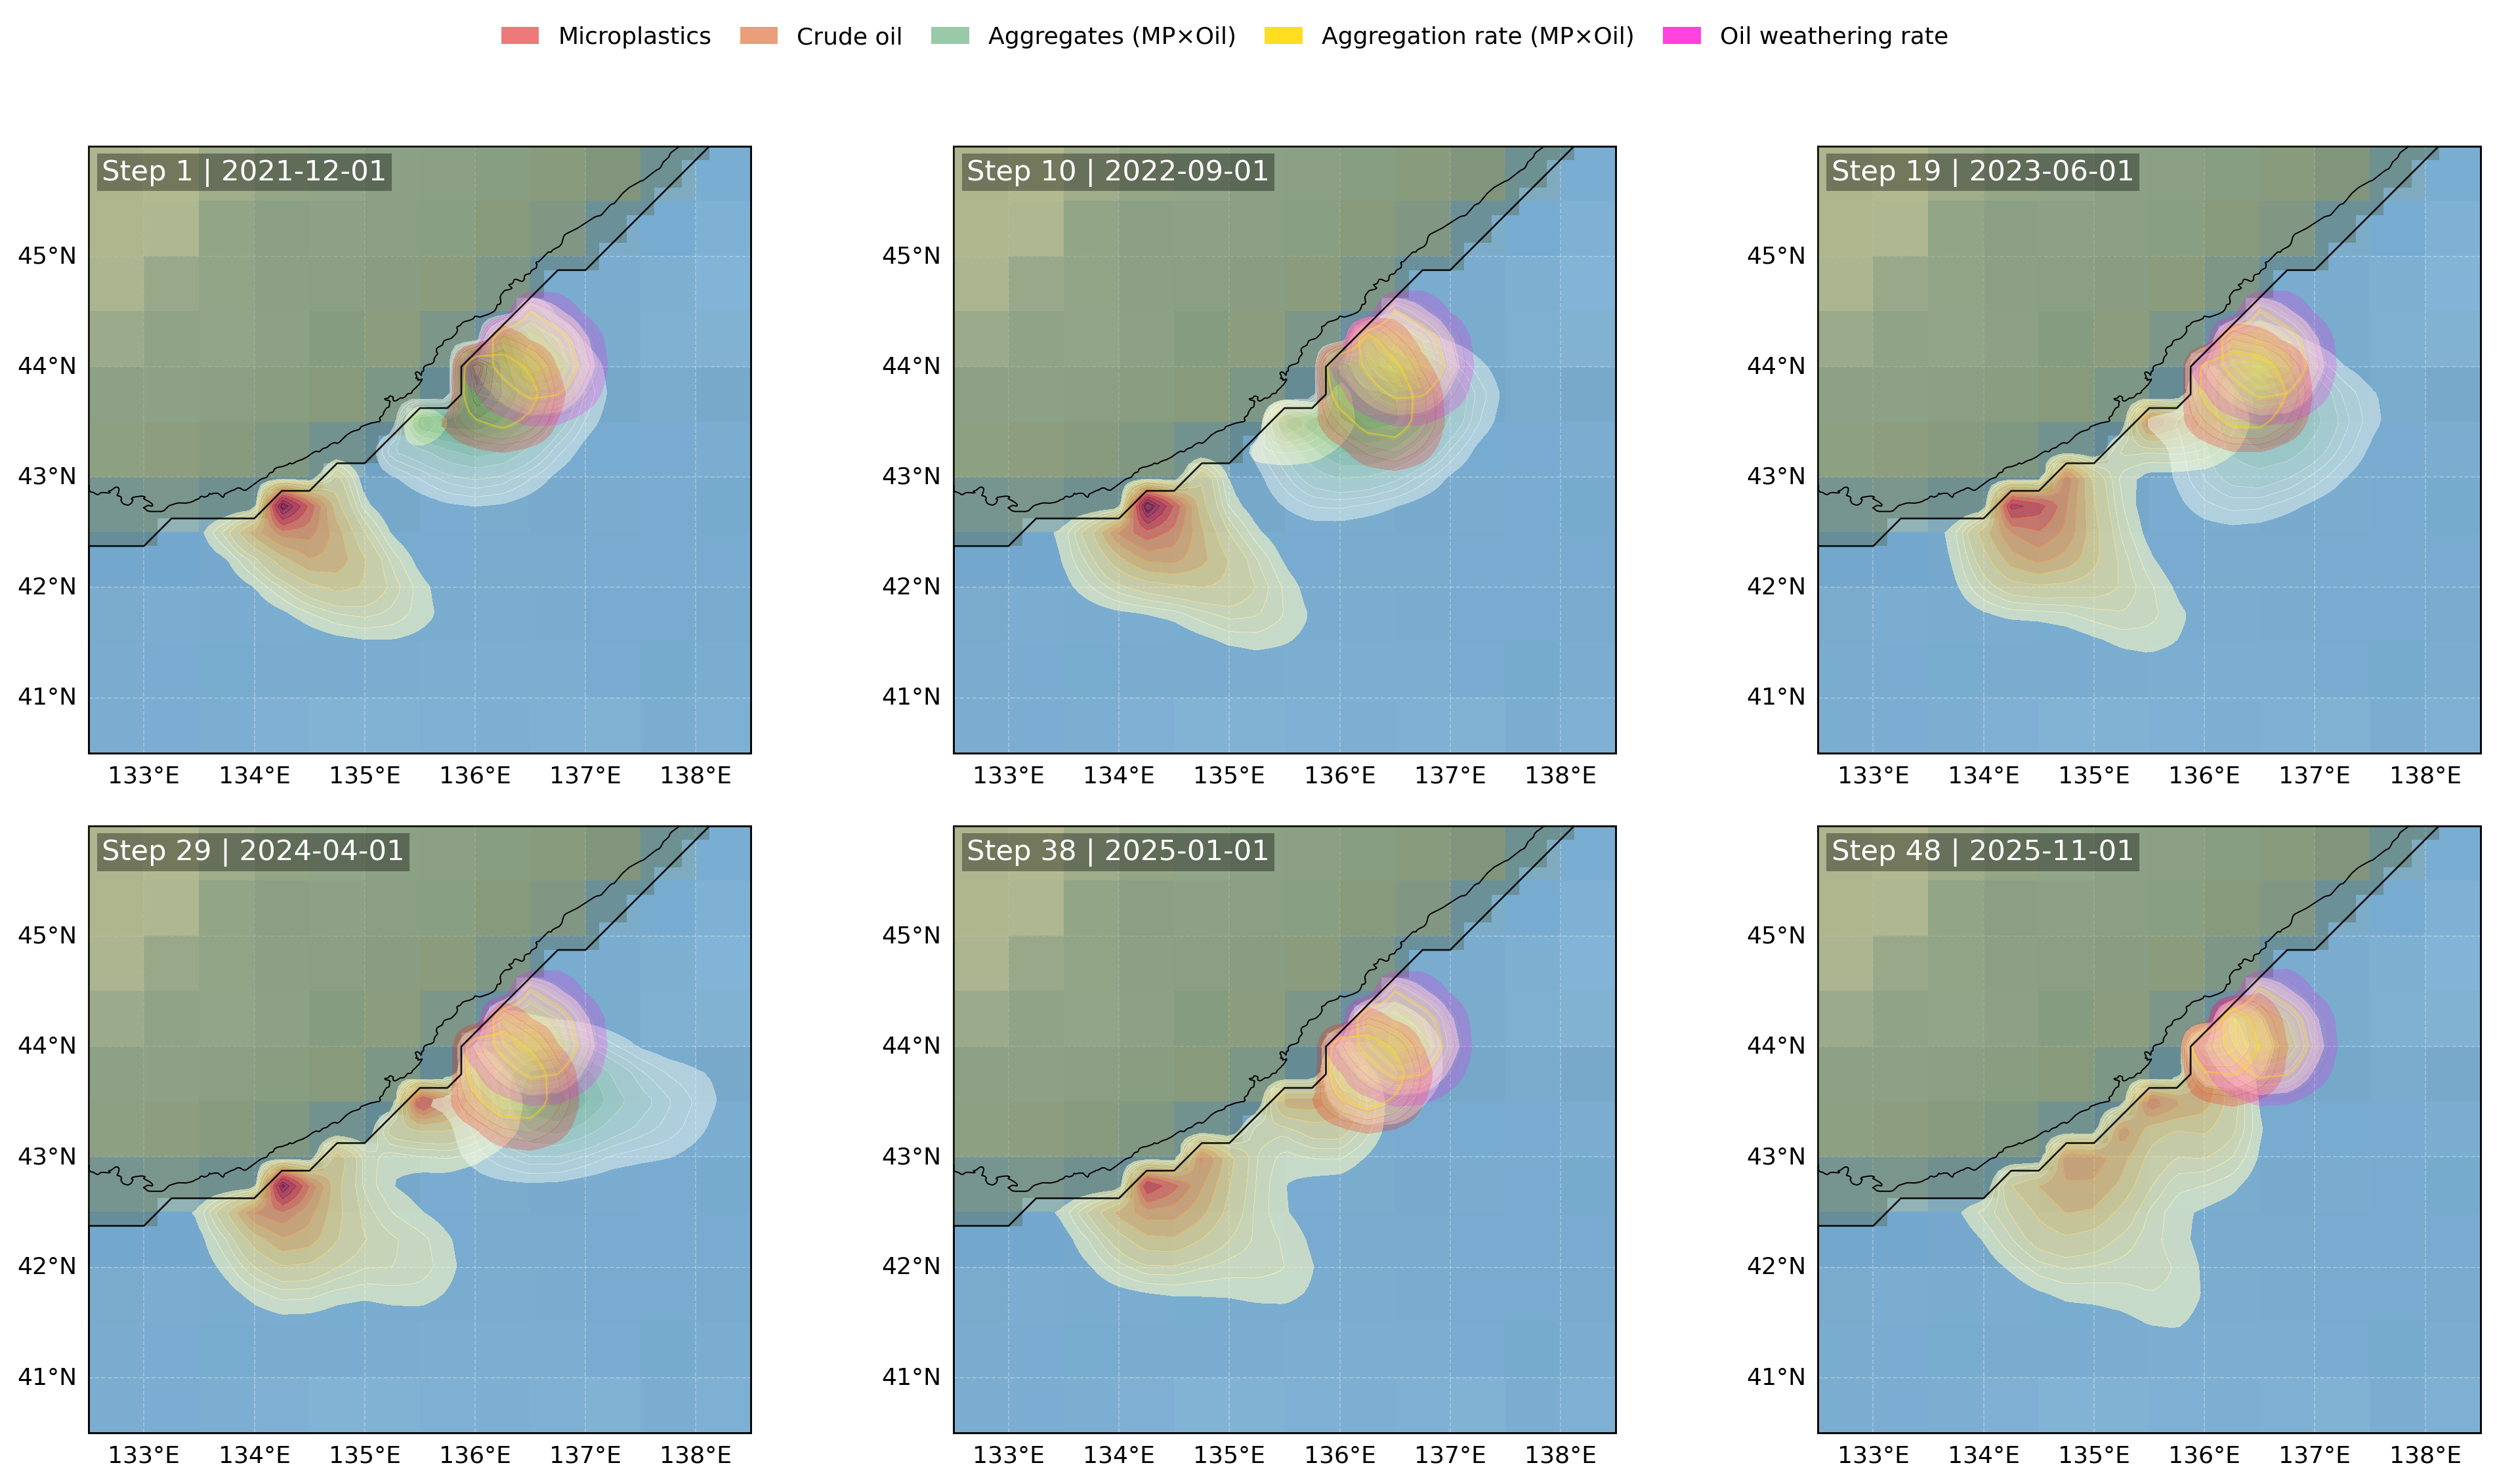
\includegraphics[width=0.98\textwidth]{figures/dataset_latest_multispecies_suite_seed03_panel.png}
\caption{Six sampled times from the dataset-driven surface multispecies proxy. The overlays show normalized microplastic, crude-oil, and aggregate fields together with aggregation and oil-weathering rates. The land mask blocks the proxy fields. Each species is normalized independently by its spatial maximum after every substep.}
\label{fig:app_multispecies}
\end{figure*}

The SPC presets use 12 sources, 8\,s dwell, and one required agent at medium difficulty; 6 sources, 6\,s dwell, and two required agents at hard difficulty.

\subsection{Optional Robot Operating System 2 (ROS 2) Jazzy bridge}

The bridge maps core $(x,y,z)=$(east, down, north) to the ROS East-North-Up (ENU) frame $(x,z,-y)$. External commands traverse the same clipping, dynamics, current, constraints, recorder, and task-update path as built-in controllers; internal-control mode can publish observations without accepting external motion commands.

\begin{table}[t]
\centering
\scriptsize
\setlength{\tabcolsep}{3pt}
\renewcommand{\arraystretch}{1.08}
\begin{tabularx}{\columnwidth}{l X}
\toprule
\textbf{Interface} & \textbf{ROS type and meaning} \\
\midrule
\texttt{/agent\_NNN/odom} & \texttt{nav\_msgs/Odometry}; ENU pose and velocity \\
\texttt{/agent\_NNN/current} & \texttt{Vector3Stamped}; ENU current \\
\texttt{/agent\_NNN/pollution} & \texttt{Float32}; local scalar probe \\
\texttt{/agent\_NNN/bathymetry} & \texttt{Float32}; positive water depth \\
\texttt{/agent\_NNN/cmd\_vel} & subscribed ENU velocity command \\
\texttt{/clock}, \texttt{/episode/metrics} & simulation time and JavaScript Object Notation episode state \\
\texttt{/reset}, \texttt{/step}, \texttt{/get\_task\_state} & \texttt{std\_srvs/Trigger} services \\
\bottomrule
\end{tabularx}
\caption{ROS 2 interface. Topic prefixes are \texttt{/oneocean/agents}; agent IDs are zero-padded.}
\label{tab:app_ros_contract}
\end{table}

The package was built and launched in a ROS 2 Jazzy container; topic discovery, frame conversion, one externally commanded step, state query, and reset completed successfully. ROS is an optional dependency.

\section{Metrics and Reproducibility Protocol}
\label{app:protocol}

\begin{table*}[t]
\centering
\scriptsize
\setlength{\tabcolsep}{4pt}
\renewcommand{\arraystretch}{1.08}
\begin{tabularx}{\textwidth}{l l l X}
\toprule
\textbf{Diagnostic} & \textbf{Budget} & \textbf{Configuration} & \textbf{Purpose} \\
\midrule
Planner diagnostic & 3 seeds per task and method & 72 episodes; stride 200; 96-token cap & Validity, fallback, completion, and failure diagnosis. \\
Dynamics diagnostic & 20 episodes per task and difficulty & 10 tasks; medium and hard; three dynamics modes & Sensitivity to vehicle dynamics. \\
Current-gain sweep & 5 seeds per task and method & 300 episodes; hard; 10 tasks; $g\in\{0,1,2\}$ & Data-current disturbance sensitivity. \\
Synthetic-tide stress & 10 seeds per task and method & 200 episodes; hard; 10 tasks; 0.45\,m\,s$^{-1}$ amplitude & Periodic-disturbance sensitivity. \\
External pollution diagnostic & 3 episodes per scene and configuration & Four scenes; two currents; two field models & Localization-model comparison. \\
External scaling & 10 episodes per scene and team size & 80 episodes; two scenes; $N\in\{2,4,8,10\}$ & Scene-backed team-size sensitivity. \\
\bottomrule
\end{tabularx}
\caption{Budgets for supplementary diagnostic studies. Headline experiment budgets remain attached to their result tables in the main paper.}
\label{tab:app_protocol_budgets}
\end{table*}

\subsection{Metric definitions}

The main paper defines Success Rate (SR), timeout-aware episode time $T$, and the action-energy proxy $E$. The additional team-level aggregate used in the result tables is the near-collision ratio
\begin{equation}
\mathrm{Coll}=\frac{1}{T_{\mathrm{ep}}}\sum_{t=1}^{T_{\mathrm{ep}}}\mathbf 1\!\left[\min_{i<j}\|p_t^{(i)}-p_t^{(j)}\|_2\le r_{\mathrm{coll}}\right].
\end{equation}
Task-specific metrics follow the definitions in Appendix Sec.~\ref{app:tasks}.

\subsection{Episode and task aggregation}

For task $k$ with $M_k$ episodes, let $s_{ke}\in\{0,1\}$ indicate success and $H_{ke}$ the timeout in seconds. The reported success rate and timeout-aware duration are
\begin{align}
\mathrm{SR}_k&=\frac{1}{M_k}\sum_e s_{ke},\\
T_k&=\frac{1}{M_k}\sum_e\left[s_{ke}t_{ke}^{\rm succ}
                         +(1-s_{ke})H_{ke}\right],
\end{align}
where $t_{ke}^{\rm succ}$ is the success time for a completed episode. The success-only duration, when reported separately, averages $t^{\rm succ}$ over successful episodes and is undefined if none succeeds.

An episode's action-energy proxy sums over both agents and executed steps:
\begin{equation}
E_{ke}=\Delta t\sum_{n=0}^{L_{ke}-1}\sum_{i=1}^{N}
                   \|\Pi_v(a_{i,n})\|_2^2.
\end{equation}
Here $L_{ke}$ is the executed step count. The proxy uses clipped commands. The near-collision ratio above uses one indicator per step, even if several agent pairs are close in that step; tables expressed in percent multiply this ratio by 100.

Station error is accumulated after each motion update. Writing $\bar d_n=N^{-1}\sum_i\|p_i^n-p_g\|_2$, its episode RMS is $[L^{-1}\sum_n\bar d_n^2]^{1/2}$. The route-tracking diagnostic analogously averages distance to the active waypoint across agents and time. It measures the waypoint-target error associated with the current route stage. For an overall success rate across $K$ tasks, the macro-average is $K^{-1}\sum_k\mathrm{SR}_k$, which gives every task equal weight. With equal episode counts this also equals the pooled episode success rate. Task-specific metrics retain their original units and are averaged within each task and configuration.

\subsection{Controller observations and decisions}

The heuristic, BC, and LLM-assisted controllers share the action interpretation and the motion update in Appendix Sec.~\ref{app:models_ros}. Heuristics track task targets, BC maps observations to velocity, and the LLM selects discrete task decisions.

\paragraph{Goal-directed control.}
For an assigned target $q_i$, the proportional controller produces
\begin{equation}
a_i=\Pi_v\!\left(k_p(q_i-p_i)\right).
\end{equation}
The navigation gain is $k_p=0.9$ and the station-keeping gain is $0.8$. Intermediate targets come from the task state: the active waypoint, assigned source, formation offset, or stage of a coordinated task. This controller corrects positional error at each step under the applied current. The pollution-localization heuristic additionally uses the agents' scalar probes to estimate a horizontal concentration gradient and coordinate exploration around the highest observed concentration.

\paragraph{Behavior Cloning.}
The observation for each training example is
\begin{equation}
o_i=[(q_i-p_i)^\top,\ y_i,\ C(p_i),\ c_{i,x},\ c_{i,z},\ e_k^\top]^\top,
\end{equation}
where $e_k$ is a one-hot task indicator. It contains seven continuous features followed by the task encoding. The policy is a multilayer perceptron with two ReLU hidden layers and a three-dimensional linear output. Feature and action means and standard deviations are estimated on the training split. With $\widehat o$ and $\widehat a$ denoting standardized values, the learning objective is
\begin{equation}
\mathcal L_{\rm BC}(\theta)=\frac{1}{3M}\sum_{m=1}^{M}
            \|f_\theta(\widehat o_m)-\widehat a_m\|_2^2.
\end{equation}
AdamW minimizes this objective. At inference the output is transformed back to action units and projected onto the permitted speed ball. The reference training configuration uses hidden widths $(64,64)$, 12 epochs, batch size 4096, learning rate $10^{-3}$, zero weight decay, and a randomly selected 10\% validation split; the trained checkpoint records its configuration and normalization statistics.

Demonstrations align the recorded command with its task target and local observations. The trajectory converter retains steps with a recorded target. For the kinematic recording convention, which stores the post-step position, it reconstructs the corresponding pre-step position as $p_n=p_{n+1}-\Delta t(a_n+c_n)$ before forming the target displacement.

\paragraph{LLM-assisted planning.}
At a planning event, the task state is summarized by the task identifier, step, team size, agent positions, and the relevant source or waypoint state. Coordinates are rounded to two decimal places. The planner returns discrete source assignments or waypoint choices, which are checked for admissible indices and task state before use. The task controller then tracks the resulting targets using the same bounded velocity control. Between planning events the current decisions remain active. Failed or invalid responses invoke the task's deterministic fallback. The diagnostic in Appendix Sec.~\ref{app:core_diagnostics} separates decision validity, fallback frequency, task completion, and inference cost, to characterize discrete planning within the closed-loop episode.

\subsection{Supplementary diagnostic budgets}



Table~\ref{tab:app_protocol_budgets} lists the supplementary diagnostic budgets and varied factors. Each study records its tier presets, controller settings, dataset indices, and environment provenance. Dataset validation and ROS interface checks are reported separately.

\subsection{Compute and run manifests}

The main paper reports the compute platform. For provenance, each run stores an integer seed, normalized configuration, task and dynamics specification snapshots, environment-product indices, software and Git state, episode metrics, and recorder streams. Aggregation scripts regenerate comma-separated-value and Markdown result tables from the recorded episode metrics.


\subsection{Extension priorities}
\label{app:limitations}

Future extensions include measured three-dimensional flow, vehicle coupling identified through Computational Fluid Dynamics (CFD) or system identification, validated pollutant transport, and ROS-in-the-loop experiments. New controllers, vehicles, and backends use the shared environment queries, declare termination conditions and metrics, and record configurations and dataset indices. They preserve the existing constraint checks and reporting formats.

\section{Additional Core-Backend Diagnostics}
\label{app:core_diagnostics}

\subsection{Dynamics-mode sensitivity}

Table~\ref{tab:app_dynamics_ablation} selects the hard-setting tasks with the largest observed dynamics sensitivity from a 20-episode-per-task diagnostic.

\begin{table}[t]
\centering
\scriptsize
\setlength{\tabcolsep}{4pt}
\renewcommand{\arraystretch}{1.10}
\begin{tabularx}{\columnwidth}{l *{3}{Y}}
\toprule
\textbf{Hard task} & \textbf{Kinematic SR} & \textbf{3DoF SR} & \textbf{6DoF SR} \\
\midrule
Formation Transit & 55\% & 50\% & 50\% \\
Surface Cleanup & 95\% & 85\% & 85\% \\
Pollution Lift & 100\% & 75\% & 75\% \\
All-task macro & 85.5\% & 81.5\% & 81.5\% \\
\bottomrule
\end{tabularx}
\caption{Selected dynamics sensitivity at hard difficulty (20 episodes per task and mode).}
\label{tab:app_dynamics_ablation}
\end{table}

Across all ten hard tasks, macro SR is 85.5\% for kinematic and 81.5\% for both 3DoF and 6DoF. Under this controller, bounded roll and pitch leave terminal success unchanged in the diagnostic, while direct kinematic integration yields higher macro success.

\subsection{Current and synthetic-tide stress}

\begin{table}[!t]
\centering
\scriptsize
\setlength{\tabcolsep}{2pt}
\renewcommand{\arraystretch}{1.08}
\begin{tabularx}{\columnwidth}{@{}>{\raggedright\arraybackslash}X l r r r r@{}}
\toprule
\textbf{Stress} & \textbf{Method} & \textbf{$N$} & \textbf{SR} & \textbf{$E$} & \textbf{Coll.} \\
\midrule
Data current, $g=0$ & Heuristic & 50 & 48.0 & 3232.5 & 5.80 \\
Data current, $g=1$ & Heuristic & 50 & 20.0 & 3371.6 & 8.24 \\
Data current, $g=2$ & Heuristic & 50 & 8.0 & 3775.0 & 9.86 \\
Data current, $g=0$ & BC & 50 & 6.0 & 1546.8 & 4.14 \\
Data current, $g=1$ & BC & 50 & 12.0 & 1807.1 & 4.96 \\
Data current, $g=2$ & BC & 50 & 4.0 & 2323.3 & 2.44 \\
Synthetic tide & Heuristic & 100 & 17.0 & 3489.2 & 6.29 \\
Synthetic tide & BC & 100 & 1.0 & 1557.6 & 6.49 \\
\bottomrule
\end{tabularx}
\caption{Hard-setting disturbance diagnostics across all ten tasks. SR and Coll. are percentages. Each data-current row contains five episodes per task. The synthetic-tide rows contain ten episodes per task, use $g=0$, and apply a 0.45\,m\,s$^{-1}$ sinusoid with a 300\,s period.}
\label{tab:app_disturbance_stress}
\end{table}

Heuristic SR decreases from 48.0\% without data-current forcing to 8.0\% at doubled current, while its energy and collision exposure increase. BC success varies non-monotonically with current gain and reaches its lowest value at $g=2$. The synthetic-tide stress also separates the methods, with 17.0\% SR for the heuristic and 1.0\% for BC.

\subsection{Planner validity, fallback, and cost}

The instrumented diagnostic contains three medium-difficulty seeds for each of eight methods and three tasks, for 72 episodes total. Tables~\ref{tab:app_llm_model_outcomes} and \ref{tab:app_llm_model_costs} aggregate each Large Language Model (LLM) across its nine episodes. Valid-plan ratio is weighted by planner calls; latency and tokens are weighted by uncached calls.

\begin{table}[!ht]
\centering
\scriptsize
\setlength{\tabcolsep}{2.5pt}
\renewcommand{\arraystretch}{1.08}
\begin{tabularx}{\columnwidth}{l *{5}{Y}}
\toprule
\textbf{LLM} & \textbf{SR} & \textbf{Calls} & \textbf{Valid} & \textbf{Fallback} & \textbf{Comp.} \\
\midrule
ChatGLM3-6B & 0.556 & 49 & 0.367 & 0.633 & 0.758 \\
Llama2-7B & 0.333 & 60 & 0.950 & 0.050 & 0.736 \\
Llama3-8B & 0.444 & 61 & 0.869 & 0.131 & 0.786 \\
Mistral-7B & 0.556 & 55 & 0.800 & 0.200 & 0.804 \\
Qwen2-7B & 0.556 & 43 & 0.814 & 0.186 & 0.790 \\
Qwen2.5-7B & 0.667 & 59 & 0.864 & 0.136 & 0.809 \\
\bottomrule
\end{tabularx}
\caption{Per-model planning outcomes across SPC, AS, and PI (nine episodes per LLM).}
\label{tab:app_llm_model_outcomes}
\end{table}

\begin{table}[!ht]
\centering
\scriptsize
\setlength{\tabcolsep}{3pt}
\renewcommand{\arraystretch}{1.08}
\begin{tabularx}{\columnwidth}{l *{3}{Y}}
\toprule
\textbf{LLM} & \makecell{\textbf{Latency}\\\textbf{ms per call}} & \makecell{\textbf{Prompt}\\\textbf{tokens per call}} & \makecell{\textbf{Output}\\\textbf{tokens per call}} \\
\midrule
ChatGLM3-6B & 1466.1 & 628.1 & 76.7 \\
Llama2-7B & 7429.6 & 633.7 & 728.7 \\
Llama3-8B & 2068.1 & 454.1 & 475.9 \\
Mistral-7B & 5150.6 & 616.5 & 676.7 \\
Qwen2-7B & 2370.6 & 603.3 & 628.6 \\
Qwen2.5-7B & 2184.5 & 600.6 & 623.9 \\
\bottomrule
\end{tabularx}
\caption{Uncached per-call planning cost in the same diagnostic.}
\label{tab:app_llm_model_costs}
\end{table}

\begin{table}[t]
\centering
\scriptsize
\setlength{\tabcolsep}{3pt}
\renewcommand{\arraystretch}{1.08}
\begin{tabularx}{\columnwidth}{l *{5}{Y}}
\toprule
\textbf{Task} & \textbf{SR} & \textbf{Valid} & \textbf{Fallback} & \makecell{\textbf{Latency}\\\textbf{ms per call}} & \textbf{Completion} \\
\midrule
SPC & 0.833 & 0.430 & 0.570 & 3199.0 & 0.972 \\
AS & 0.278 & 0.831 & 0.169 & 3602.0 & 0.758 \\
PI & 0.444 & 0.891 & 0.109 & 3337.1 & 0.611 \\
\bottomrule
\end{tabularx}
\caption{Cross-model planner diagnostics by task (six LLMs, three seeds each).}
\label{tab:app_llm_task_audit}
\end{table}

Model-level and task-level rankings also diverge: Llama2-7B attains 0.950 validity but only 0.333 SR, whereas ChatGLM3-6B attains 0.367 validity and 0.556 SR. At task level, cleanup's low valid ratio coexists with high completion because invalid or duplicate assignments can fall back to the deterministic task allocator; AS can revisit covered cells despite valid syntax, and PI still requires physical leak encounters between low-frequency plans. We report validity, fallback frequency, and task success separately.

\section{Additional External-Backend Diagnostics}
\label{app:external_diagnostics}

The external pollution study compares an analytic advected Gaussian probe with OCPNet-3D in Dam, OpenWater, PierHarbor, and SimpleUnderwater. Each combination of scene, model, and current setting uses three localization episodes; Table~\ref{tab:app_pollution_localization} therefore aggregates 12 episodes per row.

\begin{table}[t]
\centering
\scriptsize
\setlength{\tabcolsep}{2pt}
\renewcommand{\arraystretch}{1.10}
\begin{tabularx}{\columnwidth}{@{}l l *{4}{Y}@{}}
\toprule
\textbf{Scale} & \textbf{Probe} & \textbf{$N$} & \makecell{\textbf{SR}\\\textbf{(\%)}} & \makecell{\textbf{Error}\\\textbf{(m)}} & \makecell{\textbf{$\Delta$ error}\\\textbf{(m)}} \\
\midrule
1.0 & Analytic & 12 & 41.7 & 25.93 & 0.00 \\
1.0 & OCPNet-3D & 12 & 50.0 & 20.81 & $-5.12$ \\
2.5 & Analytic & 12 & 50.0 & 26.00 & 0.00 \\
2.5 & OCPNet-3D & 12 & 50.0 & 22.64 & $-3.36$ \\
\bottomrule
\end{tabularx}
\caption{Pollution-localization diagnostic over four scenes (12 episodes per row). $\Delta$ error is measured against the analytic probe at the same current scale.}
\label{tab:app_pollution_localization}
\end{table}

OCPNet-3D lowers mean localization error by 5.12\,m at nominal current and 3.36\,m under stronger current, while matching or improving aggregate success. Containment quantities are reported separately for each field model: the analytic field tracks a remaining-mass state, while OCPNet tracks grid mass. Table~\ref{tab:app_external_scaling} reports removed mass for the analytic-field team-size sweep.

\subsection{Scene-backed cleanup scaling}

\begin{table}[!ht]
\centering
\scriptsize
\setlength{\tabcolsep}{5pt}
\renewcommand{\arraystretch}{1.08}
\begin{tabular}{r r r r}
\toprule
\textbf{Agents} & \textbf{Episodes} & \textbf{SR (\%)} & \makecell{\textbf{Removed mass}\\\textbf{(kg)}} \\
\midrule
2 & 20 & 40.0 & 0.2081 \\
4 & 20 & 100.0 & 0.4302 \\
8 & 20 & 100.0 & 0.4817 \\
10 & 20 & 100.0 & 0.4886 \\
\bottomrule
\end{tabular}
\caption{Analytic-containment scaling at nominal current, aggregated over OpenWater and PierHarbor with ten episodes per scene and team size.}
\label{tab:app_external_scaling}
\end{table}

Increasing the team from two to four agents raises aggregate success from 40\% to 100\% and approximately doubles removed mass. The smaller gains from four to ten agents indicate saturation under the fixed 15\,s containment horizon.

The route and pollution results show variation across underwater scenes. Each external-backend run records the scene, current scale, dataset clock, controller settings, and observation model.


\bibliography{references}

\end{document}
